\documentclass[11pt]{jsarticle}%article??

\usepackage{../mypackage}
%\usepackage[top=10truemm,bottom=10truemm,left=15truemm,right=15truemm]{geometry}
\usepackage[]{multicol}

\usepackage{titlesec}

\titleformat*{\section}{\large\bfseries}
\titleformat*{\subsection}{\normalsize\bfseries}
\titleformat*{\subsubsection}{\normalsize\bfseries}

%
% ######## measure #########
% # mm = 1mm = 2.85pt      #
% # cm = 10mm = 28.5pt     #
% # in = 25.4mm = 72.27pt  #
% # pt = 0.35mm = 1pt      #
% # em = width of [M]      #
% # ex = height of [x]     #
% # zw = width of [Kanji]  #
% # zh = height of [Kanji] #
% ##########################
% ##################### Portrait Setting #########################
% # TOP = 1inch + ¥voffset + ¥topmargin + ¥headheight + ¥headsep #
% #     = 1inch + 0pt + 4pt + 20pt + 18pt (default)              #
% # BOTTOM = ¥paperheight - TOP -¥textheight                     #
% ################################################################
\setlength{\textheight}{\paperheight}   % 紙面縦幅を本文領域にする(BOTTOM=-TOP)
\setlength{\topmargin}{-5.4truemm}       % 上の余白を30mm(=1inch+4.6mm)に
\addtolength{\topmargin}{-\headheight}  % 
\addtolength{\topmargin}{-\headsep}     % ヘッダの分だけ本文領域を移動させる
\addtolength{\textheight}{-40truemm}    % 下の余白も30mm(BOTTOM=-TOPだから+TOP+30mm)
% #################### Landscape Setting #######################
% # LEFT = 1inch + ¥hoffset + ¥oddsidemargin (¥evensidemargin) #
% #      = 1inch + 0pt + 0pt                                   #
% # RIGHT = ¥paperwidth - LEFT - ¥textwidth                    #
% ##############################################################
\setlength{\textwidth}{\paperwidth}     % 紙面横幅を本文領域にする(RIGHT=-LEFT)
\setlength{\oddsidemargin}{-15.4truemm}  % 左の余白を25mm(=1inch-0.4mm)に
\setlength{\evensidemargin}{-15.4truemm} % 
\addtolength{\textwidth}{-25truemm}     % 右の余白も25mm(RIGHT=-LEFT)
%
%

\newif\iffigure
%\figurefaulse
\figuretrue
%select show the figure or not

\makeatletter
\def\@cite#1{\textsuperscript{#1)}}
\def\@biblabel#1{#1)}
\makeatother

\newcommand{\DATE}[3]{#1年#2月#3日} 
\newcommand{\TheDay}{\DATE{2020}{12}{01}}
\newcommand{\rHeader}{東京大学工学部航空宇宙工学科 中須賀・船瀬研究室}
\newcommand{\lHeader}{令和2年度学士論文}

%題名は重要そう
\title{コマンド及びテレメトリを用いた衛星の不具合分析支援\\に関する研究} 
\date{\TheDay} %これ日付と名前が横配置にできないかを考える
\author{03-183005 西本 慎吾}

%ヘッダの指定:
\pagestyle{fancy}

\begin{document}
%2段組みにする
\maketitle

%ここら辺のフォントを変えたい
\thispagestyle{fancy}
\lhead[\lHeader]{\lHeader} % ヘッダ左側
%\chead[偶数ページの引数]{奇数ページの引数} %ヘッダ中央
\rhead[\rHeader]{\rHeader} %ヘッダ右側
%\lfoot[偶数ページの引数]{奇数ページの引数} %フッタ左側
%\cfoot[偶数ページの引数]{奇数ページの引数} %フッタ中央
%\rfoot[偶数ページの引数]{奇数ページの引数} %フッタ右側

%\columnseprule=0.3mm

\begin{abstract}
  近年,大学や高専などの教育機関や,民間企業による超小型衛星の
開発,およびそれを利用した事業の展開が盛んになっている.
一方で,超小型衛星の信頼性の低さが問題となっている.%修正
軌道上故障に関する調査の結果
信頼性の低さの原因として,設計および製造過程における不良が多いことが分かっており,
地上試験によって不具合の改修,対策を十分に行うことが重要である.
 しかし,衛星のような複雑なシステムでは,内部の機器間で異常状態が%これおかしい
波及するため,不具合事象から
故障箇所の特定を行うことは非常に多くの知識と経験を必要とする. 
 そこで,本研究ではコンポーネント間の接続関係モデル,情報
 伝達の経路モデルを用いて衛星の故障候補の
 検証方法(確認事項,打つべきコマンド)を人間の判断を支援する
 指標と共に提示することで,不具合分析を支援する手法を提案する.
 本手法では,簡易的な衛星モデルに対して実践することで
 コマンドによる故障箇所の特定を効率的に行えること,設計の不備を発見
することにつながることを確認した.
%多分背景以外のところをもう少し詳細に述べたほうがいい気がする.
\end{abstract}

\begin{multicols}{2}
  \section{序論}
  \vspace{-1zh}
  \subsection{研究背景}
  \vspace{-1zh}
  超小型衛星開発に大学などの参加が増加している中,
  信頼性の低さが問題となっている\cite{Langer2016}.
  軌道上故障の調査の結果,衛星の故障原因の多くは設計・製造過程に起因するものである\cite{Venturini2017}
  ことが分かっており,それらの多くは地上試験によって確認することができるものである
  という結果が出ている\cite{SAITO2011}.
 
  %設計・製造における不良が軌道上故障の多くを占めている現状がある.
  %解決するためには地上試験において,設計上の不良を発見し十分に改修しなけらばならない.

  \begin{figure}[H]
    \centering
      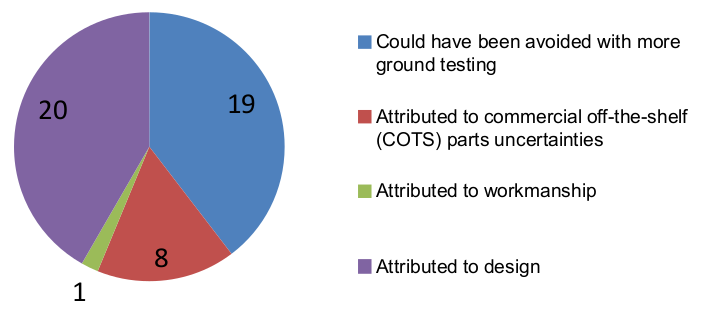
\includegraphics[height=3.0cm]{../figure/cause_of_failure.png}
      \caption{超小型衛星の故障原因に関する調査結果\cite{Venturini2017}}
      \label{fig:cause_of_failure}
  \end{figure}
  
 % \vspace{-1zh}
  %地上試験の不備が発生する原因として地上試験で改修を行う難しさがあるということを言いたい
  \subsection{問題提起}
  \vspace{-1zh}
  以上より,地上試験での不具合分析が不十分になっていることが,超小型衛星の
  信頼性の低さの原因の一つである.地上試験での不具合分析を十分に行うためには
  以下の2点の作業に高い知識と経験が必要とされる.
  %地上試験における検証が不十分になっている原因の一つとして故障候補の洗い出しや故障箇所の
 %特定作業が知識依存になっていることが挙げられる.
  \begin{itemize}
    \item 故障候補の網羅的洗い出し
    \item 故障候補の切り分け作業
  \end{itemize}
  まず,故障候補を洗い出す作業はFTAを用いて不具合事象から考えられる故障モード
  を網羅的に洗い出すことを行うが,衛星は内部機器の物理的相互作用が複雑
  であるため,人による思い付きでは網羅的に行うことは難しい.
  %アクティブセンシングを行うことを述べる.それが安全である必要がある
  また,切り分け作業は衛星から得られる情報を元に
  衛星の安全を確保しながら行う必要があり,不具合事象から衛星の状態を
  十分に想像できなければ安全な切り分け作業を行うことができない.
  %故障仮説の網羅的洗いに関する研究についてもう少しまとめる
これに対して,下表\ref{tab:previous_research}に示すように,
故障候補の洗い出しを網羅的に行う研究が盛んにおこなわれている.
一方で,不具合分析の一つの大きな課題である検証過程に関して取り組んだものは少ない.
%一方で,故障候補の切り分ける過程に関して取り組んだ研究は少ない.
%安全に行う必要があることを言いたい.

\vspace{-1zh}
%比較軸が微妙過ぎる
\begin{table}[H]
  \centering
  \caption{不具合分析手法の比較}
  \label{tab:previous_research}
   \scalebox{0.9}{
     \begin{tabular}{cccccc} \hline%もう少し示し方を考える.
        手法&故障網羅性&手法の目的%&モデル複雑度%専門家の知識が必要という点で?
        \\ \hline
        GDE&低&故障仮説生成%&低
        \\ %見てないし無くてもいいかも
        GDE+\cite{Struss1989}&中&故障仮説生成%&中
        \\
        網状故障解析\cite{Yamaguchi2014}&中&異常モード洗い出し%&高
        \\
        故障オントロジー\cite{Kitamura1999}&高&故障仮説生成%&高
        \\
        本手法&中%低かもしれない.接続関係しか見れていない
        &故障箇所特定支援%&中
        \\ \hline
     \end{tabular}}
\end{table}
\vspace{-1zh}
\subsection{本研究の目的}
%別にここの文言をまねする必要はない
以上より,次の機能を持った不具合事象から故障候補の切り分けまでの作業を
体系化し,不具合分析経験の少ない人を支援する手法を提案する.
%コマンドとテレメトリをベースにしたものを対象にしていることを言った方がいいかもしれない
  \begin{itemize}
  \item 異常テレメトリから故障候補を生成する.
  \item 故障候補を確認するためのコマンドおよびテレメトリを提案する.
  \item 上の探索結果に関して優先度を人間に提示する.
\end{itemize}
上記の機能を実現するために,本種研究では以下の3点の構築を目的とする.%???
\begin{itemize}
  \item 衛星内部機器の接続関係モデル及び情報伝達経路モデル
  \item 故障箇所の特定を行うために必要なコマンド及びテレメトリの探索アルゴリズム
  \item 人間の判断を支援するためのコマンドの評価指標
\end{itemize}
\vspace{-1zh}
\section{モデルベース不具合分析手法の仕様}
\vspace{-1zh}
\subsection{不具合分析アルゴリズム}
\vspace{-1zh}
本手法による
不具合分析の流れを下図\ref{fig:fault_diagnosis_flow}に示す.
人間と対話的に故障箇所の特定を行う仕様となっており,これにより
実機の情報をシステムにフィードバックしながら故障箇所を絞り込むことができるようになる.
%ちょっと文字が小さい
\begin{figure}[H]
  \centering
    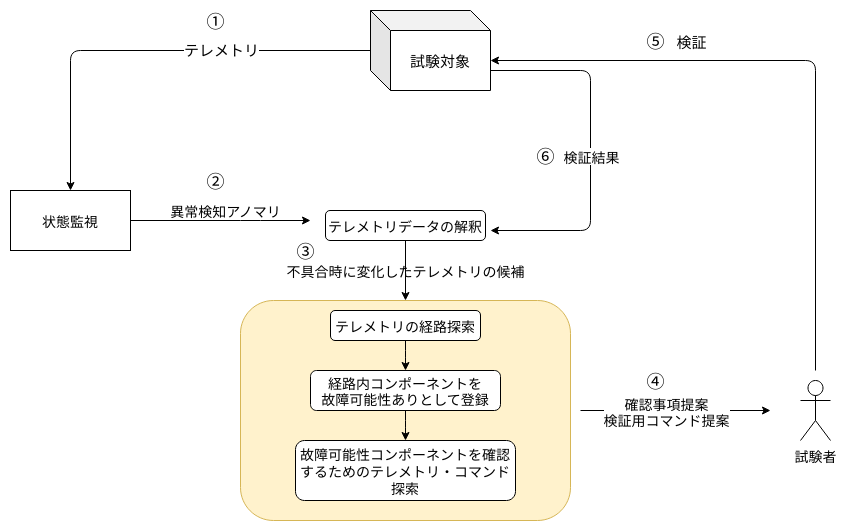
\includegraphics[height=5.8cm]{../figure/fault_diagnosis_flow.png}
    \caption{本手法による不具合分析の流れ}
    \label{fig:fault_diagnosis_flow}
\end{figure}

\subsection{モデル}%オントロジーやけどね
上述したアルゴリズムで故障個所の特定を行うために
使用するモデルに関して以下に示す.

%結局これ機能の話と接続関係の話が混ざってるから適切な分類なのかはわからない
\subsubsection{コンポーネント間接続関係モデル}
來村ら\cite{Kitamura01}は拡張デバイスオントロジーとして,機器間の接続関係を
「ポート」と「導管」という概念を用いて表現している.
これを元に,コンポーネントの接続関係を表す「リンク」(表\ref{fig:link})を定義した.各リンクには正常確率
を属性として持ち,これによって以降に述べるコマンドの評価を行うことを可能にしている.
また,表\ref{fig:compo}のように各コンポーネントがリンクを属性として持ち,コマンドの情報伝達
で使用するリンクとテレメトリの情報伝達で使用するリンクを区別している.
\begin{table}[H]
  \centering
  \caption{リンク定義}
  \label{fig:link}
\end{table}
\vspace{-3zh}
\begin{figure}[H]
  \centering
    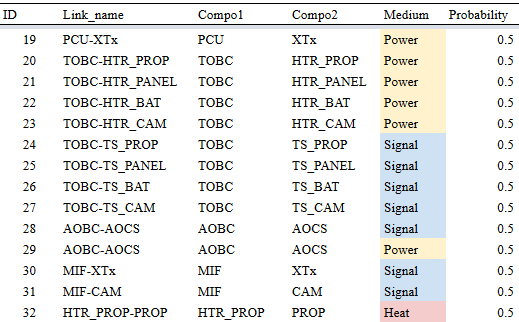
\includegraphics[height=5.0cm]{../figure/link_definition_resume.png}
\end{figure}
\vspace{-2zh}

\begin{table}[H]
  \centering
  \caption{コンポーネント定義}
  \label{fig:compo}
\end{table}
\vspace{-3zh}
\begin{figure}[H]
  \centering
    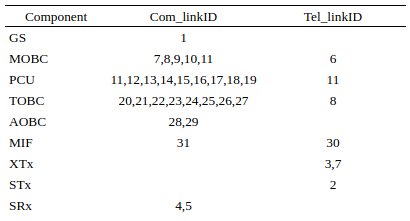
\includegraphics[height=3.5cm]{../figure/compo_link_resume.png}
\end{figure}

\vspace{-2zh}
\subsubsection{情報伝達経路モデル}
%次に,コマンドとテレメトリによる情報伝達経路のモデルに関して示す.
以下の表\ref{fig:COM},\ref{fig:TEL}のようにコマンドおよびテレメトリを定義した.
それぞれ情報伝達の経路を上述のリンクによって表現している.また,コマンドには属性として
影響を与えるテレメトリ及びコマンドの種別を与えており,これによってコマンドを送信した際に
得られる情報を類推している.\\%説明が曖昧過ぎる気がするな
また,テレメトリのモデルでは,テレメトリが変化するトリガの種類を指定しており,
これによって故障箇所特定に必要な情報取得のために取る行動を決めることができる.
ここでは簡単のため,軌道運動などによる状態変化は考慮せず,時間とコマンドだけによる
状態遷移を考えている.

\begin{table}[H]
  \centering
  \caption{コマンドモデル}
  \label{fig:COM}
\end{table}
\vspace{-3zh}
\begin{figure}[H]
  \centering
    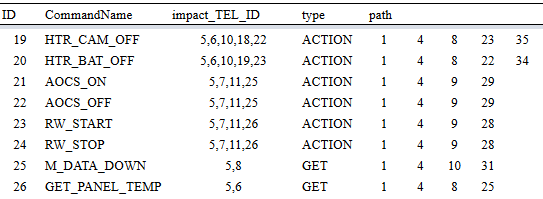
\includegraphics[width=8cm]{../figure/COM_resume.png}
\end{figure}

\begin{table}[H]
  \centering
  \caption{テレメトリモデル}
  \label{fig:TEL}
\end{table}
\vspace{-3zh}
\begin{figure}[H]
  \centering
    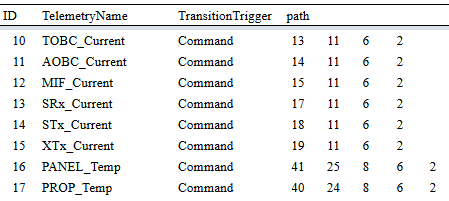
\includegraphics[height=3.5cm]{../figure/TEL_resume.png}
\end{figure}

%機能に関しては必要ないかもしれない.とりあえず必要なのはつながりと経路.
%それに確率があることを説明する
コマンドおよびテレメトリの機能モデル%これは違うかも
でも状態量の更新に関して説明するために必要.

\vspace{-1zh}
\subsection{評価指標の提案}
本手法の対象は地上試験における支援であるが,不具合分析に利用する情報の粒度が
コマンドとテレメトリのみであるため,軌道上不具合発生時の故障箇所特定にも
利用可能である.そこで,以下では地上試験及び軌道上での運用時の両方で重要となる
指標を提案し,本手法が両状況で使い分け可能なフレームワーク%枠組みでええくない?
であることを示す.
\vspace{-1zh}
%なんでこの2点を指標にするのかを説明する.
  \subsubsection{衛星の生存への副作用}
  まず,生存への副作用を示す指標として,以下の3点を与える.
  \begin{itemize}
    \item コマンドを打つ前の電力状態と,コマンドを打つことによって発生する電力消費量
    \item 姿勢変化を起こすか否か
    \item コマンド送信によって変化するテレメトリの数
  \end{itemize}
  前者2点の電力と姿勢による制約から来る指標は運用時に特有のものであり,コマンドを打つことで
  衛星の安全を脅かすことがないように危険な動作を明示的に示すことで,
  未熟な運用者による誤ったコマンド送信を防ぐ目的がある.
  また,不具合発生時は衛星の状態に対する把握が不十分であるため,衛星の状態を大きく変化
  させるコマンドは危険であるといえる.そのため,コマンドによって発生する状態変化
  の大きさを定量的に示す指標として3点目の指標を与えている.
\vspace{-1zh}
\subsubsection{故障候補切り分け能力}
  運用時は可視時間が限られており,その時間内に不具合の改修を行わなければ
  ミッションが失敗するような,時間制約を考慮した不具合分析を行う場面が考えられる.
  その際には,少ないコマンド数で効率的に故障個所の特定を行えることが望ましい.
  

 まず,一つのコマンドで切り分けられる故障候補の数を表す指標に関して述べる.
 %この図は使っているようで使えていない
 以下の図\ref{fig:route}に示すような故障候補(太矢印)がある場合を考える.
 あるリンク($l_i$)の状態を確認するためにはその経路($\text{R}_j$)内にある他のリンク
 が正常である必要がある.よって,
 \begin{eqnarray}
  P(l_{i} | \text{R}_j) &=& \prod_{m\in\mathbb{F}_j,i\neq m} P(l_{m} = \text{normal})
 \end{eqnarray}
 の確率でリンク$l_i$を確認できる.ここで$\mathbb{F}_j$は$\text{R}_j$内の故障候補
 リンクの集合,$P(l_{m} = \text{normal})$は上述した各リンクの正常確率を表している.
 $P(l_{i} | \text{R}_j)$はコマンドが形成する各径路すべてに対して求まるので
 それらの最大値を取りコマンド(C$_k$)による$l_i$の確認可能性は
\begin{eqnarray}
  P(l_i|\text{C}_k) &=& \max  \{ P(l_i|\text{R}_{j})\}
\end{eqnarray}
となる.\\
また,これが各リンクに対して求められるのでそれらの平均を取り,「平均確認可能性($P_m(\text{C}_k)$)」
及びC$_k$によって確認可能なリンクの数を表す「確認可能リンク数($E(\text{C}_k)$)」が以下のように求まる.
ここで,$\mathbf{N_{F_k}}$
はコマンドが形成する経路内にある故障候補の数を表す.
\begin{eqnarray}
  P_m(\text{C}_k) &=& \frac{1}{\mathbf{N_{F_k}}}\sum_{i=1}^{\mathbf{N_{F_k}}}
  P(l_i|\text{C}_k) \label{eq:Pm Ck} \\
  E(\text{C}_k) &=& \mathbf{N_{F_k}}P_m(\text{C}_k) =
   \sum_{i=1}^{\mathbf{N_{F_k}}}P(l_i|\text{C}_k) \label{eq:E Ck}
\end{eqnarray}

  %これも文字小さい.この図で説明する必要があるのか?
  \begin{figure}[H]
    \centering
       \begin{tabular}{c}
          \begin{minipage}{0.30\hsize}
          \centering
          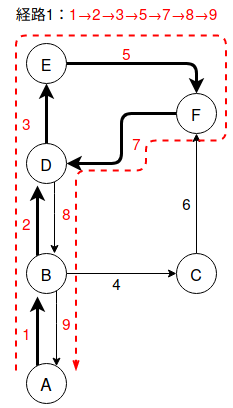
\includegraphics[height=4.5cm]{../figure/route1.png}
           %  \caption{}
             \label{fig:route1}
          \end{minipage}
          \begin{minipage}{0.30\hsize}
          \centering
          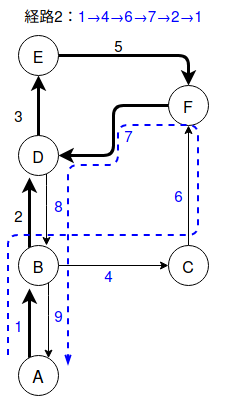
\includegraphics[height=4.5cm]{../figure/route2.png}
          %\caption{}
             \label{fig:route2}
          \end{minipage}
          \begin{minipage}{0.30\hsize}
             \centering
             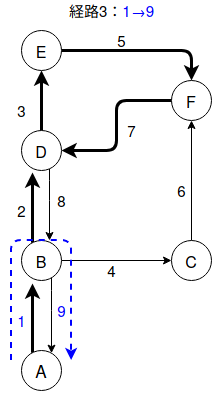
\includegraphics[height=4.5cm]{../figure/route3.png}
             %\caption{}
                \label{fig:route2}
             \end{minipage}
       \end{tabular} 
       \caption{故障候補とそれを確認するための情報伝達経路の例}%ここも変えたほうがいいかも
       \label{fig:route}
 \end{figure}
%図がどこに入るかでスペースを調整する必要がある.
式(\ref{eq:Pm Ck}),(\ref{eq:E Ck})がどちらも高いコマンドを選択することで,
一つのコマンドでより多くの故障候補を絞り込むことが可能である.\\
  次に,あるコマンドから検証を開始した時に,最終的に故障箇所の特定を行うまでにかかる
  コマンドの総数に関して述べる.%述べる系いらんかな
以下の図\ref{fig:all_process}に示すように,あるコマンドによる検証を考えると
各テレメトリの結果によって残る故障候補が変化する.この時,故障候補が残っている場合には
それに応じたコマンドの探索を行う必要がある.
各テレメトリが正常値を示すか否かは各リンクごとの正常確率を用いて以下の式(\ref{eq:P_TEL_normal}),
(\ref{eq:P_TEL_abnormal})のように算出でき,これを元に図\ref{fig:all_process}の各Caseへの確率が求まる.
ここで,$\text{T}_j$はIDが$j$のテレメトリを表しており,経路の添え字と対応している.
\begin{figure}[H]
  \centering
    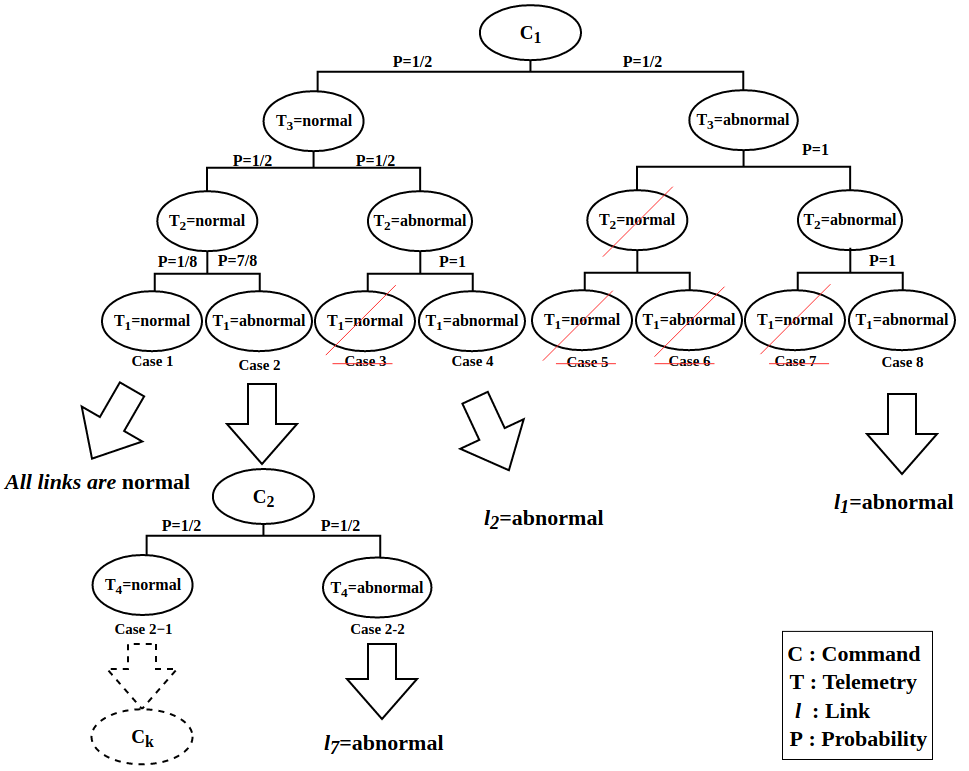
\includegraphics[height=6.5cm]{../figure/all_process.png}
    \caption{検証プロセスの全体像}
    \label{fig:all_process}
\end{figure}
\begin{eqnarray}
  P(\text{T}_j = \text{normal}) &=& \prod_{i\in\mathbb{F}_j} P(l_i = \text{normal}) \label{eq:P_TEL_normal}\\
  P(\text{T}_j = \text{abnormal}) &=& 1 - P(\text{T}_j = \text{normal}) \label{eq:P_TEL_abnormal}
\end{eqnarray}
各Caseに応じて,最終的故障箇所を切り分けるまでのコマンドの総数が異なるので,それによって
以下の式(\ref{eq:N Ck})のように期待値が求められ,
%P(Case i)に関しては表式がめんどくさすぎるので書かない
\begin{eqnarray}
  N(\text{C}_k) &=& \sum_{\text{Case }i\in\mathbb{C}} P(\text{Case }i) N_{\text{Case }i} \label{eq:N Ck}
\end{eqnarray}
これを「検証コマンド総数」と定義する.ここで,$\mathbb{C}$は検証が終了した結果の各場合(Case)の集合である.%日本語が変かも
検証コマンド総数が少ないコマンドを選択することによって,全体的に
かかるコマンドの数の期待値が小さい検証プロセスを選択することができる.


\subsubsection{評価指標の使い分け}
%表にする方がいいか?
以下の表\ref{tab:indicator usage}に以上で示した指標をどのように使い分けるかに関して
示す.地上試験時は電力と姿勢による制約はほぼ考えなくてよい.
効率性を重視したい場合は$P_m(\text{C}_k)$,$E(\text{C}_k)$が高く,
$N(\text{C}_k)$が小さいコマンドを選択すれば良い.

\begin{table}[H]
  \centering
  \caption{地上試験と運用時での指標の優先度(3段階,降順,\textcolor{red}{赤}:安全重視,黒:効率重視)}
  \label{tab:indicator usage}
  \scalebox{0.8}{
    \begin{tabular}{c|ccc|cccc} \hline %段作って効果と副作用に分けたほうがいいかも
      &電力&姿勢&影響TEL数&$P_m(\text{C}_k)$&$E(\text{C}_k)$&$N(\text{C}_k)$ \\ \hline
      地上試験&-&-&\textcolor{red}{2},1&\textcolor{red}{1},3&\textcolor{red}{1},3&\textcolor{red}{1},3\\
      運用時&\textcolor{red}{3},1&\textcolor{red}{3},1&\textcolor{red}{2},1&\textcolor{red}{1},2&\textcolor{red}{1},2&\textcolor{red}{1},3\\ \hline
    \end{tabular}}
\end{table}
%これ〇だとよくわからない.状況によるからなもう少し場合分けして示せばいいのか?
%地上試験と運用での分類で変わるところは電力と姿勢だけ,安全目か効率重視かで分ける?
%数字で優先度を見せたほうが分かる?


  \section{提案手法による実践と評価}
  \subsection{対象問題設定と実践結果}
  テストケースに用いる衛星モデルを以下に示す.
  \begin{figure}[H]
    \centering
      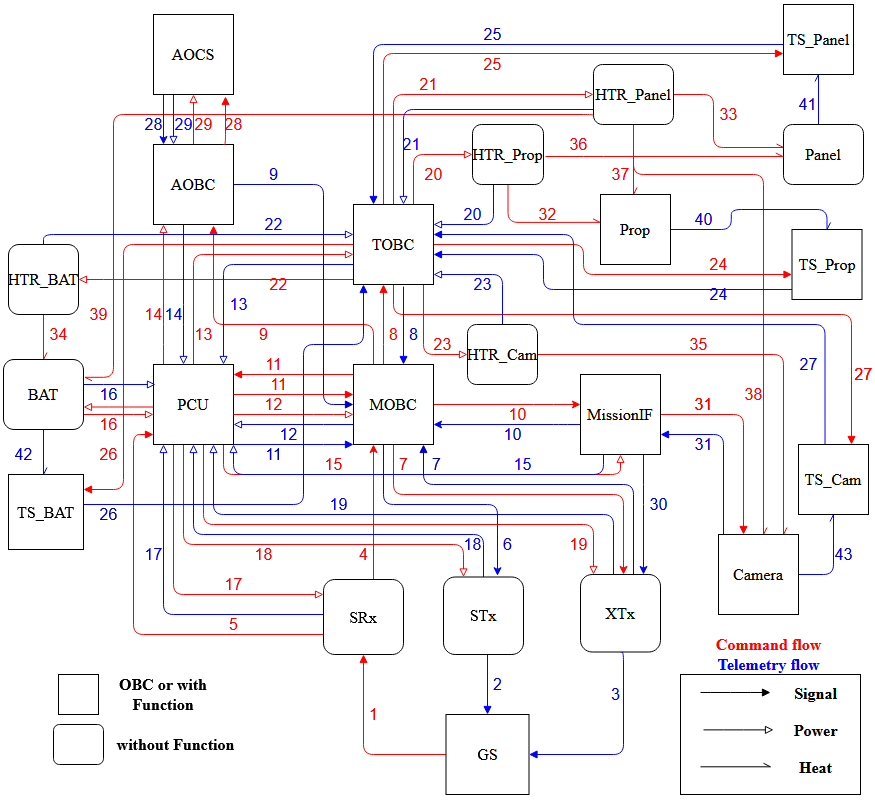
\includegraphics[height=7.0cm]{../figure/satellite_diagram.png}
      \caption{簡易衛星モデル}
      \label{fig:satellite}
  \end{figure}
  
  実践例での対象故障.
  複数の事例を確認して,どうだったかという結果も欲しい


  実践例として上手く特定ができるものと,できないものを示す.
 \begin{itemize}
   \item ヒータの接触不良に関して
   \item コンポーネントの故障などに関して(そもそものテレメトリが発行されていない場合など)
 \end{itemize}
  \subsection{}

  \section{結論}
  \subsection{本研究で得られた知見}%知見なのか?まとめ的な
本研究ではモデルを用いてコマンドによる故障箇所特定のプロセスを体系化する手法を提案し,
テストケースを用いてその有効性を検証した.

  本手法を用いて最終的な故障箇所の特定を行うのは難しい.どちらかというと
  不具合分析過程を体系化して,それを用いたコマンドの選択をすることによって
  故障箇所の推論に必要な情報を集めるような働きをしていると言える.

  テレメトリを発行している機器の故障の場合は,そのコンポーネントから
  の情報ラインに冗長系がなければかなり多くの故障候補が残ってしまう.
%多分複数の検証結果を総合して判断するような処理が必要になるんやろな

  \subsection{今後の展望}
 今後,接続関係の異常だけでなく,実問題に近い故障状態も扱えるようにするために,
 扱う状態量をより詳細にモデル化していく必要がある.また,テレメトリと状態量の対応付けを考えることによって
 異常状態をリンクとして表現するのではなく,各コンポーネントの機能の異常を特定できると考えている.

 また本手法では,簡易的に故障候補の洗い出しを情報伝達の経路のみに絞っていたが,
 \cite{}で提案されているオントロジーを用いることで,細かい粒度の特定を目標に行っていく必要がある.

 今回の例では,モデルの構築を手作業により行ったが,実ミッションでの適用を考慮すると手作業によるモデル構築は
 現実的ではない.今後ある程度の事前定義情報からモデル化を自動化することを目標にする.
  
 リンクの正常確率として,より実機で用いているコンポーネントの信頼度に近い値を考えることで,
 モデルが複雑になった際により効率的な故障箇所特定を行えると考えている.

  
  \bibliographystyle{junsrt} %plain, acm, alpha とか
  \bibliography{../Ref} 

\end{multicols}
\end{document}